\section{Corpora}
\subsection{Selection criteria}

For the purposes of this paper, it was desirable that the corpora used be:
\begin{itemize}
    \item representative of what language learners strive for
    \item available in many languages
    \item for background corpora: Document-level
    \item freely accessible
\end{itemize}

\subsection{Corpora used}
\begin{description}
	\item[OpenSubtitles Parallel Corpus]
	      This set of corpora contains parallel corpora:
	      Corpora which has text segments in one language aligned with the presumed translation of the segment in a second language.
	      Its sentences are generated from subtitles from the popular subtitle sharing platform \textit{OpenSubtitles} (https://www.opensubtitles.org/) and undergo various preprocessing and filtering steps as described in \cite{lisonOpensubtitles2016ExtractingLarge2016}.
	      These include:
	      \begin{enumerate}
		      \item Enforcing universal UTF-8 character encoding.
		      \item
		            Splitting and joining of sentences from their original subtitles blocks (the segments which appear on screen when watching the movie with its subtitle).
		            One such block may contain multiple sentences, or only a partial one.
		            There is thus a n-to-m-relationship between the blocks and sentences.
		      \item Checking and correcting possible spelling issues, especially ones arising from OCR (Optical character recognition) errors.
		      \item From available subtitles, identifying the subtitle pair which is most likely to be accurate in its alignments and free from errors such spelling, taking into account metadata such as user ratings of subtitles.

	      \end{enumerate}
		  One advantageous aspect of this corpus is that is contains many sentences that are sequential, which means we can generate a Next Sentence Prediction dataset from it (add hedging here since not all lines in corpus are sequential and even within the same movies there may will be pauses in the subs).
		  This corpus has been used to train machine translation models such as OPUS-MT \cite{tiedemannOPUSMTbuildingOpenTranslation2020}, a freely available set of transformer models for translation, including between low-resource languages. \todo{Not completely correct, the pipeline uses data from OPUS, not necessarily or specifically from OpenSubs}
		  While it is possible to reconstruct which movies the subtitle lines came from from information contained in the corpus, it is unfortunately not clear how these movies were selected in the first place.

	\item[Leipzig Wortschatz Corpora]
		Available in x languages

		But: data quality issues, methodology might be outdated

		\cite{goldhahnBuildingLargeMonolingual2012}
	\item[CCMatrix / NLLB]

\end{description}

The full process, as illustrated by the authors, can be seen in figure \ref{fig:opensubs pipeline}
As of 2025, the latest version of the corpus (v2018) contains aligned subtitles of 62 languages between each other.

\begin{figure}[H]
	\centering
    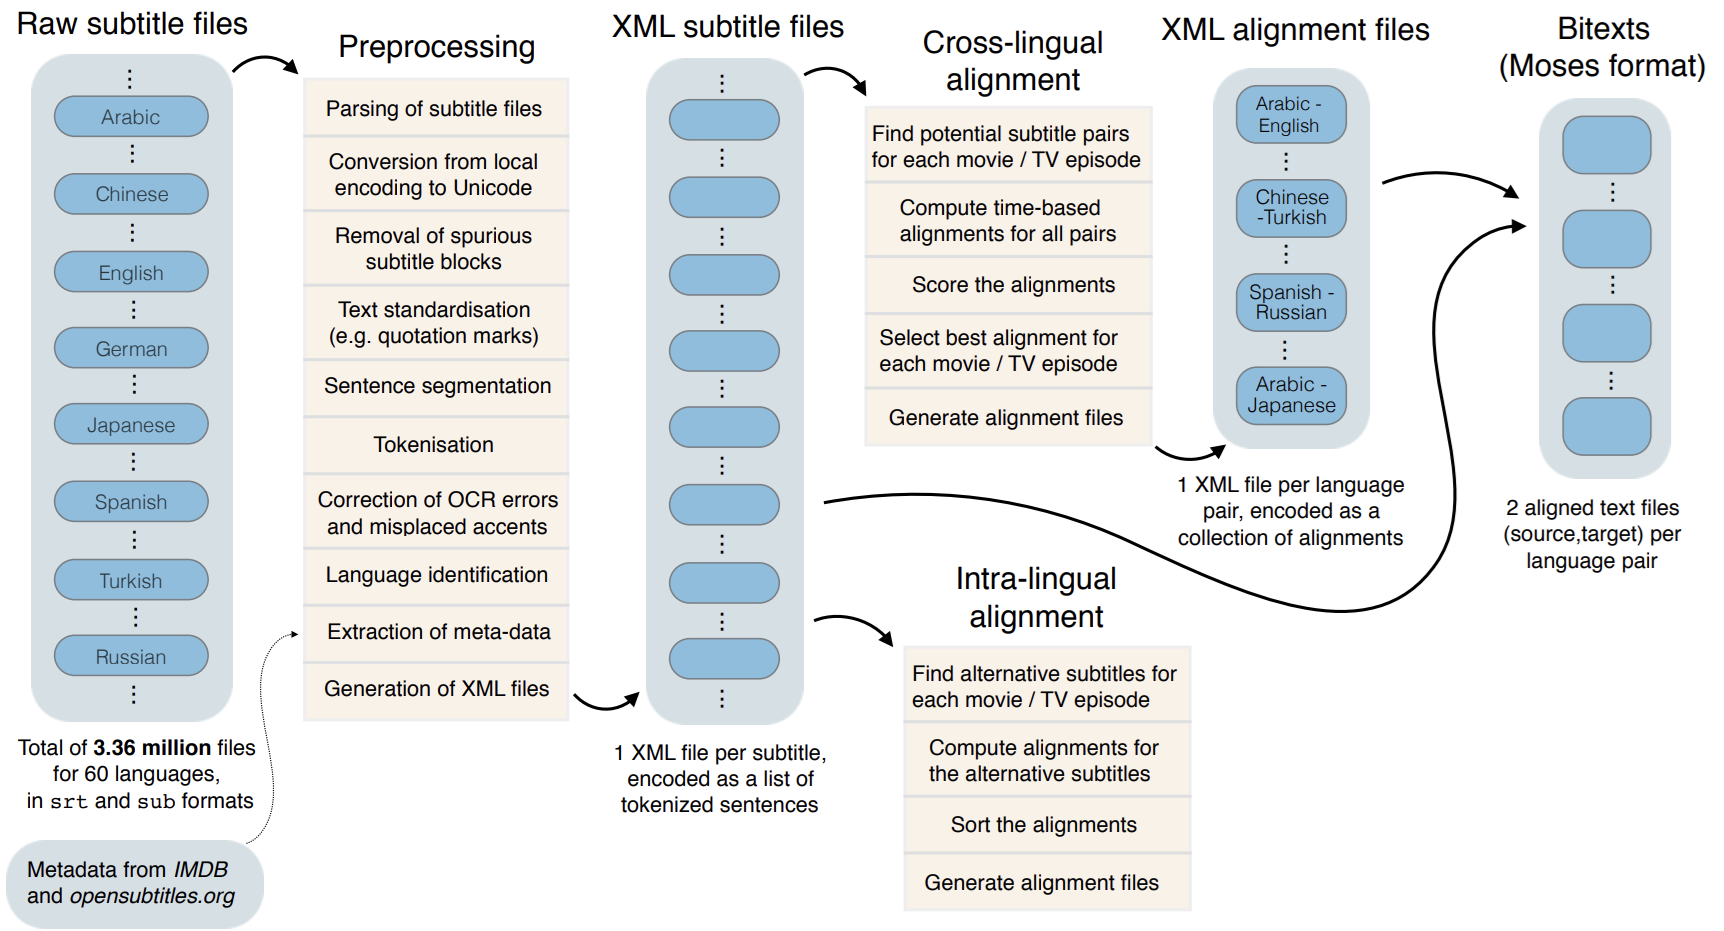
\includegraphics[width=\textwidth]{opensubs_corpus_processing.png}
	\caption{The pipeline producing the OpenSubtitles parallel corpus}
    \label{fig:opensubs pipeline}
\end{figure}

\section{Sources for existing lists for comparison}
It may be useful to compare the lists generated by the various approaches with existing word lists from educational materials:
Textbooks often feature chapters with word lists, or sentences which can be converted to word lists with a tokenizer.
The purpose is to have a point of comparison, to see if generated lists agree with existing lists, and find reasons for differences.

\begin{itemize}
	\item Language learning textbooks

	\item Language learning applications
	      \begin{itemize}
		      \item Duolingo: While Duolingo is the most popular language learning application as of 2024, it does not publish its word lists or course contents that is free of cost and easily convertible to a format that can be processed with NLP tools.
		      \item Rosetta Stone: Rosetta Stone publishes Course contents on its website. While the contents take the form of sentences, these can be converted to word lists by using a tokenizer on the contents and creating a list in the order in which they appear in the texts.
	      \end{itemize}
\end{itemize}


\section{Data Augmentation}
Data Augmentation was not used to gain additional data.
While in recent years data augmentation methods have become popular for training AI models in NLP, most of these would have either no or a detrimental effect on the methods employed in this paper:
Some of these methods include \cite{pellicerDataAugmentationTechniques2023}:
\begin{description}
	\item[Character level]
	      Introducing character swaps to data is a method used to train the model to noise in the data, but in our case, would only add noise to the results.
	\item[Word level]
	      There exist techniques to switch words for synonyms or swap words in the sentences to create noise.
	      As with noise on the word level, adding words in inappropriate places is undesired for our use case.
	      Swapping words for synonyms would also prove detrimental, as this would skew the statistics away from the natural word distribution found in the human-generated source texts.
\end{description}
Higher level techniques suffer from the same issues.
For this reason, the data is left in its "natural state" for our purposes.
